

Para implementar este scheduler, debemos mantener $n$ cantidad de colas, donde $n$ es la cantidad de cores del procesador. Además, como cuando entra un proceso nuevo debemos asignarlo al procesador con menos procesos totales, nos conviene tener un vector que nos dice cuantos procesos totales tiene cada core. Como siempre, tenemos los quantums de cada procesador, y el tiempo restante que tiene cada tarea de cada core. 

Finalmente, tenemos un diccionario, cuyas claves son tareas y sus significados son cores, que nos dice para cada proceso bloqueado, a que core le corresponde. Necesitamos esto para sabes, cuando un proceso se desbloquea, a que core asignarselo.

Entonces, cuando entra un nuevo proceso, buscamos cual es el core con menos procesos actuales, y lo asignamos ahí. Cuando un proceso termina, lo que hacemos es fijarnos en la cola de cada core cual es el proceso que sigue.

Cuando un proceso se bloquea, lo definimos en el diccionario nombrado anteriormente; y cuando se desbloquea, buscamos en el diccionario a que core tiene que ir y borramos su entrada.

\subsection{Escenario 1}

La versión de Round Robin que no migra nucleos es beneficiosa en conjuntos de tareas que usan intensivamente el CPU y la memoria durante mucho tiempo. Como la memoria se usa intensivamente, migrar cores es costoso porque se pierde todo lo que estaba cacheado. 

El lote que diseñamos consiste en 3 tareas, cada una empieza un segundo despues de la otra, y cada una usa el procesador por 30 unidades de tiempo.

\begin{lstlisting}
TaskCPU 30
@1:
TaskCPU 30
@2:
TaskCPU 30
\end{lstlisting}


\begin{figure}[H]
\caption{Ejemplo de un lote de tareas que solo usa CPU en Round Robin 1}
\label{fig:ej8-11}
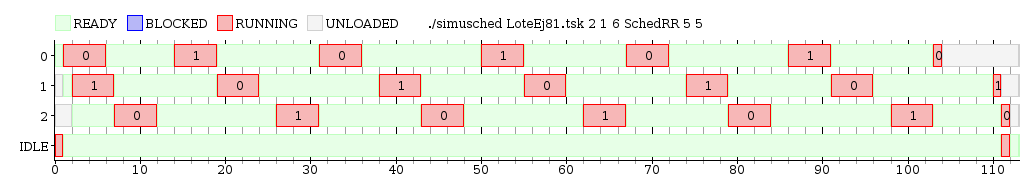
\includegraphics[width=0.9\columnwidth]{imgs/ej8-1rr.png}
\end{figure}

\begin{figure}[H]
\caption{Ejemplo de un lote de tareas que solo usa CPU en Round Robin 2}
\label{fig:ej8-12}
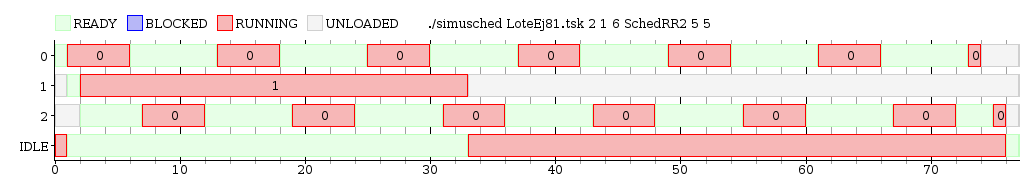
\includegraphics[width=0.9\columnwidth]{imgs/ej8-1rr2.png}
\end{figure}

Las métricas que analizaremos serán la eficiencia (tiempo en el que el cpu está corriendo las tareas sobre tiempo total) y el throughput.

Como se ve en la figura \ref{fig:ej8-11}, la eficiencia de el algoritmo de scheduling que migra nucleos no es tan alta, dado que la migración de nucleos ocurre muy seguido y se debe pagar un costo muy alto cada vez. Por esta misma razón, el throughput de este algoritmo es también bajo.

Por otro lado, como se ve en la figura \ref{fig:ej8-12}, la eficiencia de el algoritmo de scheduling que no migra nucleos (si no fuera por el idle del final, que se solucionaria simplemente poniendo igual cantidad de tareas en cada nucleo) es mucho más alta. Esto se debe a que al no migrar nucleos, se aprovecha el cache del core y no es se paga el costo de perderlo. Por esta razón, el throughput del algoritmo es más alto que antes, terminando las tareas en casi la mitad del tiempo que el anterior algoritmo.

\section{Escenario 2}

Ahora veamos que pasa si hay una tarea que se bloquea por mucho tiempo, una que lo usa por muy poco tiempo y otras 2 que requieren usar CPU por un poco más de tiempo.

\begin{lstlisting}
TaskIO 1 70
TaskCPU 50
@1:
TaskCPU 5
TaskCPU 50
\end{lstlisting}

\begin{figure}[H]
\caption{Ejemplo de un lote de tareas que se bloquean y usan CPU en Round Robin 1}
\label{fig:ej8-21}
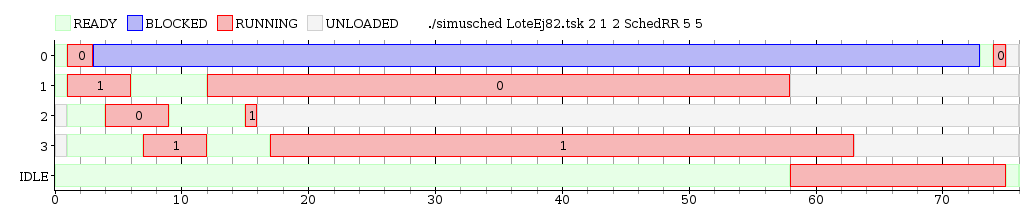
\includegraphics[width=0.9\columnwidth]{imgs/ej8-2rr.png}
\end{figure}

\begin{figure}[H]
\caption{Ejemplo de un lote de tareas que se bloquean y usan CPU en Round Robin 2}
\label{fig:ej8-22}
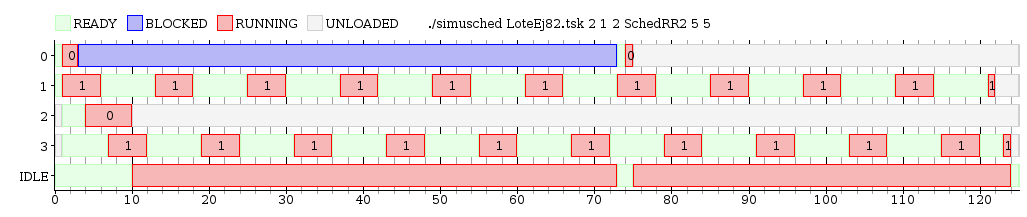
\includegraphics[width=0.9\columnwidth]{imgs/ej8-2rr2.png}
\end{figure}


Como se ve en la figura \ref{fig:ej8-21}, el rendimiento y el throughput de esta versión es altisimo. Esto se debe a que, cuando se bloquea un proceso, el algoritmo puede correr en paralelo las 2 tareas demandantes de CPU en paralelo totalmente.

Sin embargo, en la versión del algoritmo que no permite migración entre procesadores, en la figura \ref{fig:ej8-22} todo cambia. Al no poder migrar tareas entre núcleos, cuando la tarea 2 termina, y la tarea 0 está bloqueada, el procesador 1 tiene una carga muy alta, mientras que el procesador 0 esta totalmente ocioso. Por esta razón, la eficiencia es mucho más baja que antes, y en consecuencia, el throughput es mucho más bajo.



